
\subsection{Primeras métricas: MaxDif y  \texorpdfstring{$MaxDif_g$}{MaxDifg}} 

\begin{frame}[t]\frametitle{Primeras métricas: MaxDif}
Para cada palabra $\omega$ y cada par de provincias $p_1$ y $p_2$, podemos calcular el cociente entre la frecuencia máxima de $\omega$ en ambas provincias y la frecuencia mínima:

\begin{equation}
  \label{eq:maxDif} 
  maxDif(\omega,p_1,p_2) = \frac{f_{max}(\omega,p_1,p_2)}{f_{min}(\omega,p_1,p_2)}
\end{equation}

Desventajas:  
\begin{enumerate}
    \item \label{1} Un valor para cada par de provincias.
    \item \label{2} No se considera la dispersión de los valores en todas las provincias.
\end{enumerate}

\end{frame}

\begin{frame}[t]\frametitle{Primeras métricas: $MaxDif_g$}

Considerando las frecuencias de una palabra $\omega$ sobre todas las provincias, definimos:

\begin{equation}
 maxDif_g(\omega) = \frac{f_{max}^\prime(\omega)}{f_{min}^\prime(\omega)}
 \label{eq:maxDifg}  
\end{equation} 
donde $f_{max}^\prime(\omega)$ es la frecuencia máxima de la palabra $\omega$ entre las frecuencias de todas las provincias y $f_{min}^\prime(\omega)$ es la frecuencia mínima distinta de $0$.

Con $maxDif_g$ se resume en un único valor la contrastividad de la palabra, sin embargo sigue sin considerar la distribución de las frecuencias.


\end{frame}

\subsection{Entropía y valor de la información}

\begin{frame}[t]\frametitle{La entropía de la información}
    
% La entropía nos brinda un valor que indica qué tan uniforme es la distribución de las frecuencias de cada palabra. 
\only<1->{
    Sea $\mathbf{p}=(p_1,\ldots, p_n)$ un vector de probabilidad puntual. Es decir, $p_i\geq 0$ y $\sum_{i=1}^np_i=1$. 

    Definimos la entropía de $\mathbf{p}$ siendo
    \begin{equation}
    H(\mathbf{p})=-\sum_{i=1}^n \log(p_i)p_i.
    \end{equation}
}

\only<2>
{
    \begin{exampleblock}{Dime que tan uniforme eres y te diré cuanta entropía tienes} Las palabras utilizadas más uniformemente en las distintas provincias como \textit{de} o \textit{que} aportan menos información que la palabra \textit{celular}. 
\end{exampleblock}
}

\only<3>
{
    \begin{block}{Observaciones}
        \begin{enumerate}
            \item $H(\mathbf{p})=0$ si y solo si $\mathbf{p}$ esta concentrada en un unico punto: existe $i$ tal que $p_i=1$ y $p_j=0$, para todo $j\not=i$. 
            \item La funci\'on $H$ se maximiza tomando $\mathbf{p}$ equiprobable: $p_i=1/n$, para todo $i$. 

        \end{enumerate}

    \end{block}
}
\end{frame}



\begin{frame}[t]\frametitle{Valor de la información}
    Zanette y Montemurro definieron al \textit{valor de la información de una palabra} como
 \begin{equation}
  \Delta I_w(\omega) = p(\omega) \,  (\widehat{H}(\omega) - H(\omega))  =  p(w) \, \Delta{H(\omega)}
 \end{equation}
siendo $p(\omega)$ la frecuencia total de la palabra en el texto.


\end{frame}

\subsection{Valores contrastivos}
\begin{frame}[t]\frametitle{Valor contrastivo sobre las palabras}
    \begin{alertblock}{Valor contrastivo sobre las palabras}
        \begin{equation}
            I_w(\omega) = norm_{w}(\omega) \cdot (\widehat{H}_{w}(\omega) - H_{w}(\omega))
            \label{eq:iw}
        \end{equation}
        donde $norm_w$ sirve para normalizar sobre la cantidad de ocurrencias de la palabra.
    \end{alertblock}

    \begin{block}{Observaciones}
        \begin{itemize}
            \item Si una palabra se dice muchas veces el valor de $I_w(\omega)$ es más alto.
            \item Si dos palabras se dicen la misma cantidad de veces, la palabra que tenga una dispersión más heterogenea será la de mayor valor contrastivo sobre las palabras.
        \end{itemize}
    \end{block}

\end{frame}

\begin{frame}[t]\frametitle{Robusteciendo métrica: valor contrastivo sobre las personas}
    \only<1>{
    ¿Y si algunas palabras tienen un $I_w$ alto debido a pocas personas que las mencionan constantemente?
    \medskip
    
    \alert{Hay que tener en cuenta a la distribución de la cantidad de personas que mencionan cada palabra en las provincias.}
    }

    \only<1-2>{
        \begin{alertblock}{Valor contrastivo sobre las personas}
        \begin{equation}
            I_p(\omega) = norm_p(\omega) \cdot (\widehat{H}_p(\omega) - H_p(\omega))
            \label{eq:iu}
        \end{equation}
        donde $norm_p$ sirve para normalizar sobre la cantidad de personas que mencionan la palabra $\omega$.
    \end{alertblock}
    }

    \only<2>{
        \centering
        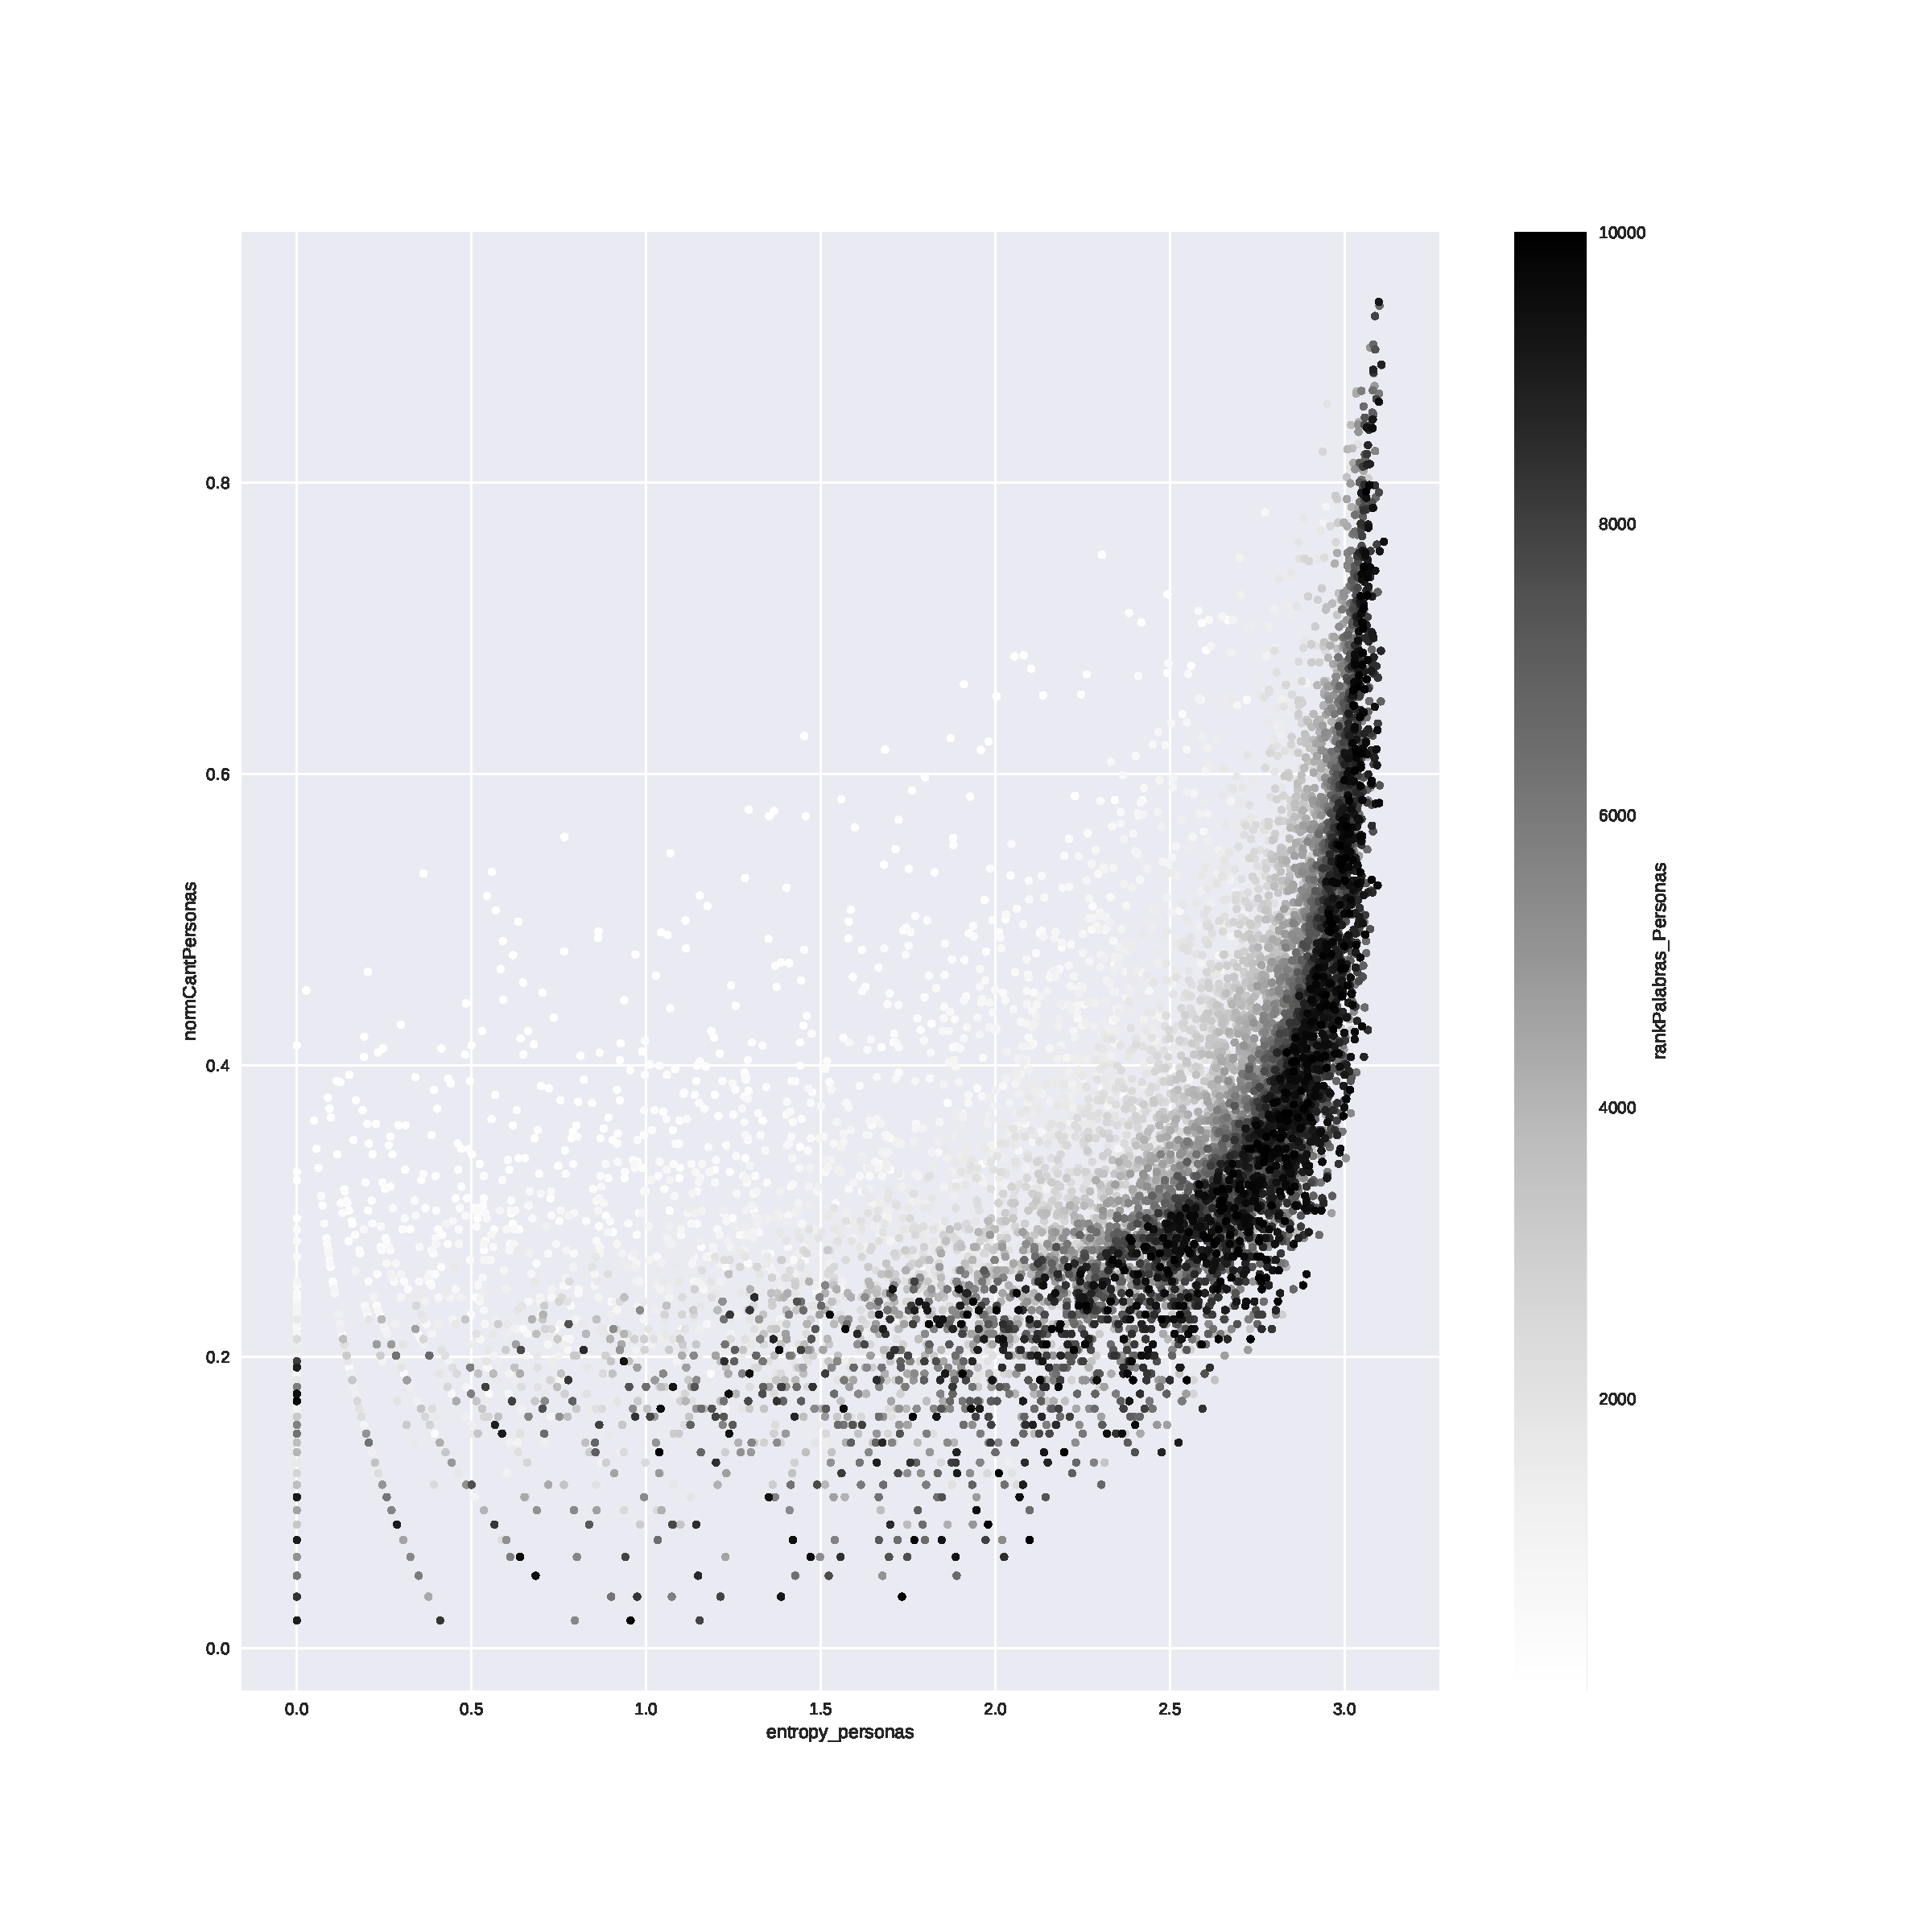
\includegraphics[width=.55\textwidth]{../src/images2/entropiaPersonasxNormCantPersonas.pdf}
    }

    
\end{frame}

\begin{frame}[t]\frametitle{Valor de contrastividad}
    \begin{block}{Valor de contrastividad}
    Como nos interesa tanto la distribución de la cantidad de ocurrencias de cada palabra, como la de la cantidad de usuarios que la menciona, definimos   
    \begin{equation}
    I(\omega) =  I_w (\omega) \cdot I_p(\omega)
    \label{eq:ivalor}
    \end{equation}
    \end{block}    

    \begin{columns}
        \begin{column}{.7\linewidth}
        \includegraphics[width=.9\textwidth]{../src/images/PropAcumSinCandidatas.pdf}
        \end{column}
        \begin{column}{.3\linewidth}
        Proporción de ocurrencias acumulada según la muestra de palabras. % El número de la leyenda indica la cantidad de palabras contrastivas elegidas para la muestra respectiva, siempre seleccionando las más contrastivas según la métrica.
        \label{fig:propAcum}
        \end{column}
      \end{columns}
   

\end{frame}